\documentclass{beamer}

\usepackage[T1]{fontenc}
\usepackage{inputenc}

\usepackage{amsmath}
\usepackage{listings}
\lstset{
  basicstyle=\footnotesize,
  language=Caml,
  showstringspaces=false,
}


\usetheme{Boadilla}
\usecolortheme{dolphin}
\useoutertheme{infolines}


\setbeamertemplate{footline}
{
  \leavevmode%
  \hbox{%
  \begin{beamercolorbox}[wd=.333333\paperwidth,ht=2.25ex,dp=1ex,center]{author in head/foot}%
    \usebeamerfont{author in head/foot}\insertshortauthor%~~\beamer@ifempty{\insertshortinstitute}{}{(\insertshortinstitute)}
  \end{beamercolorbox}%
  \begin{beamercolorbox}[wd=.333333\paperwidth,ht=2.25ex,dp=1ex,center]{title in head/foot}%
    \usebeamerfont{title in head/foot}\insertshorttitle
  \end{beamercolorbox}%
  \begin{beamercolorbox}[wd=.333333\paperwidth,ht=2.25ex,dp=1ex,right]{date in head/foot}%
    \usebeamerfont{date in head/foot}\insertshortdate{}\hspace*{2em}
    \insertframenumber{} / \inserttotalframenumber\hspace*{2ex}
  \end{beamercolorbox}}%
  \vskip0pt%
}

\title{mi.TLS}
\author{Nicolas Kox and Maxime Puys}
\date{\today}


\begin{document}

\begin{frame}
    \maketitle
\end{frame}

\section{Problem presentation}

\begin{frame}
  \frametitle{\emph{Protocol rupture}}

  Aims to create a device able to filter communications in SCADA\\
  Aim to get a high level of certification\\
  \vfill
  
  Need to support various protocols : SFTP, Modbus, OPC-UA\\

\end{frame}



\begin{frame}
  \frametitle{Constraints}

  Need to provide a critical embedded software, and thus avoid 
  
  \begin{itemize}
    \item Run-Time Errors (RTE)
    \item Code or command injection
    \item Authorizations bypass
    \item ideally also Denial of Service (a bit more difficult)
  \end{itemize}

  In addition, updating embedded software is quite painful, technically and monetarily\\
  Thus, we must provide strong security guarantees before deployment

\end{frame}




\section{Security properties offered by mi.TLS}

\begin{frame}
    \tableofcontents[currentsection]
\end{frame}

\begin{frame}
    \frametitle{Languages used}
    \begin{block}{F\#}
        Programming language.\\
        Functionnal language such as OCaml on top of Microsoft .NET.
        Very rich type system.
    \end{block}

    \begin{block}{F7}
        Refinement typechecker for F\#.
        Idea: Asserts on types.
    \end{block}

    \begin{block}{Fournet et al. [2011]}
        Probabilistic variant of F7.
        Framework for cryptographic verification of protocols.
        Adds the concept of secrecy.
    \end{block}
\end{frame}

\begin{frame}
    \frametitle{Architecture}
    
    \begin{itemize}
        \item mi.TLS is implemented in a modular way.
        \item Each module is proven separately and then linked together using type refinements.
        \vfill
        \item Crypto is assumed safe and relies on common assumptions (RSA-PMS and DH-PMS).
        \item Cryptographic primitives come from cryptolibs such as OpenSSL and BouncyCastle.
    \end{itemize}
\end{frame}



\begin{frame}[fragile]
    \frametitle{F\# example}

    \begin{lstlisting}
(* Parametric hash algorithm (implements interface) *)
let hash' alg data =
    match alg with
    | NULL    -> data
    | MD5SHA1 -> (CoreHash.md5 data) @| (CoreHash.sha1 data)
    | MD5     -> (CoreHash.md5    data)
    | SHA     -> (CoreHash.sha1   data)
    | SHA256  -> (CoreHash.sha256 data)
    | SHA384  -> (CoreHash.sha384 data)

let hash alg data =
  let h = hash' alg data in
  let l = length h in
  let exp = hashSize alg in
  if l = exp then h
  else Error.unexpected "Hash of an unexpected size"
    \end{lstlisting}
\end{frame}

\begin{frame}[fragile]
    \frametitle{F7 example}

    \begin{lstlisting}
private val hash': a:hashAlg -> bytes -> b:bytes

val hash: a:hashAlg -> bytes -> b:bytes{Length(b)=HashSize(a)}
    \end{lstlisting}
\end{frame}

\begin{frame}[fragile]
    \frametitle{Fournet et al. [2011] example}

    \begin{lstlisting}
ask !si,p,g,gs,a,k,t.
    B(t) = B(si.init_crand) @| B(si.init_srand)
        @| DHEParamBytes(p,g,gs) /\
    Length(si.init_crand) = 32 /\
    Length(si.init_srand) = 32 /\
    Sig.Msg(a,k,t) /\
    k = Cert.SigPKCert(si.serverID,a) =>
    (DHGroup.PP(p,g) /\ DH.HonestExponential(p,g,gs))
    \end{lstlisting}
\end{frame}

\begin{frame}
    \frametitle{Security properties offered by mi.TLS in general}

    \begin{block}{Properties}
        Privacy and integrity of a bytestream sent over TLS.
    \end{block}
    \vfill
    \begin{block}{Adversary}
        A probabilistic, polynomial adversary even using chosen adaptative plaintext and ciphertext learns nothing on the content  and cannot cause them to accept any other content.
    \end{block}
\end{frame}

\begin{frame}
    \frametitle{Proof of these properties}

    Such results are expressed using indistinguishability games.
    
    \begin{block}{Example}
        \begin{columns}[T]
            \begin{column}[T]{.4\textwidth}
                \[\begin{array}{l}
                    Game~OW-PCA =\\
                    pk,sk       \leftarrow keygen()\\
                    k^{'},c^{'} \leftarrow enc(p^{'},pk)\\
                    k           \leftarrow A^{PCO}(pk, c^{'})\\
                    return (k = k^{'})
                \end{array}\]
            \end{column}
            \begin{column}[T]{.4\textwidth}
                \[\begin{array}{l}
                    Oracle~PCO(p,k,c)   =\\
                    if p \not\in P~or~k = \bot then\\
                    ~~~~return \bot\\
                    k^{'}               \leftarrow dec(p,sk,c)\\
                    return (k^{'} = k)
                \end{array}\]
            \end{column}
        \end{columns}
    \end{block}
\end{frame}




\begin{frame}
    \frametitle{Security properties on the handshake}

    \begin{itemize}
        \item Uniqueness: avoid replay attacks.
        \vfill
        \item Verified safety: if a client trusts both the negotiated algorithm and the server certificate then it can deduce that its session with the server is safe.
        \vfill
        \item Agile key derivation: the keys used are indistinguishable from a random fresh key.
        \vfill
        \item Agreement: for a complete and safe handshake, there is a safe handshake in the other role such that their two protocol instances agree on the same assignement to all variables.
    \end{itemize}
\end{frame}


\begin{frame}
  In order to complete proof, some TLS features have been disabled :
  \begin{itemize}
  \item weak algorithms : MD5, DES, PKCS\#1
  \item TLS compression : avoid CRIME attacks
  \end{itemize}
  \vfill
  New features have been implemented to avoid newly found attacks
  \begin{itemize}
  \item renogociation and resumption are now related to previous session : avoid triple-handshake attack
  \item error buffer is checked after handshake : avoid partial error messages that could change fatal errors to warning
  \item length-hinding of the blocks size
  \end{itemize}

\end{frame}



\section{Deployment}


\begin{frame}
    \tableofcontents[currentsection]
\end{frame}


\subsection{Using mi.TLS}




\begin{frame}
    \frametitle{Architecture}
    
    \begin{table}
        mi.TLS\\
        $\uparrow$\\
        F\# / F7\\
        $\uparrow$\\
        .NET (Mono on UNIX)\\
        $\uparrow$\\
        OS (Windows or UNIX)\\
        $\uparrow$\\
        Micro-kernel\\
        $\uparrow$\\
        Hardware\\
    \end{table}
\end{frame}

\begin{frame}
    \frametitle{What we succeded until now}

    \begin{table}
        mi.TLS\\
        $\uparrow$\\
        F\# / F7 v3.0\\
        $\uparrow$\\
        Mono v3.2.8 (Open-source .NET for UNIX)\\
        $\uparrow$\\
        Ubuntu 14.04.1 (i686)\\
        $\uparrow$\\
        Linux 3.13.0-24-generic\\
        $\uparrow$\\
        Virtualbox machine\\
    \end{table}
\end{frame}

\begin{frame}
    \frametitle{Can we use mi.TLS on a micro-kernel?}
    
    \begin{table}
        \begin{tabular}{c}
            .NET (Mono on UNIX)\\
            ~\\
            {\Huge $\uparrow$ ?}\\
            ~\\
            Micro-kernel\\
        \end{tabular}
    \end{table}
    
\end{frame}

\begin{frame}
\frametitle{.NET CVE (no comment)}

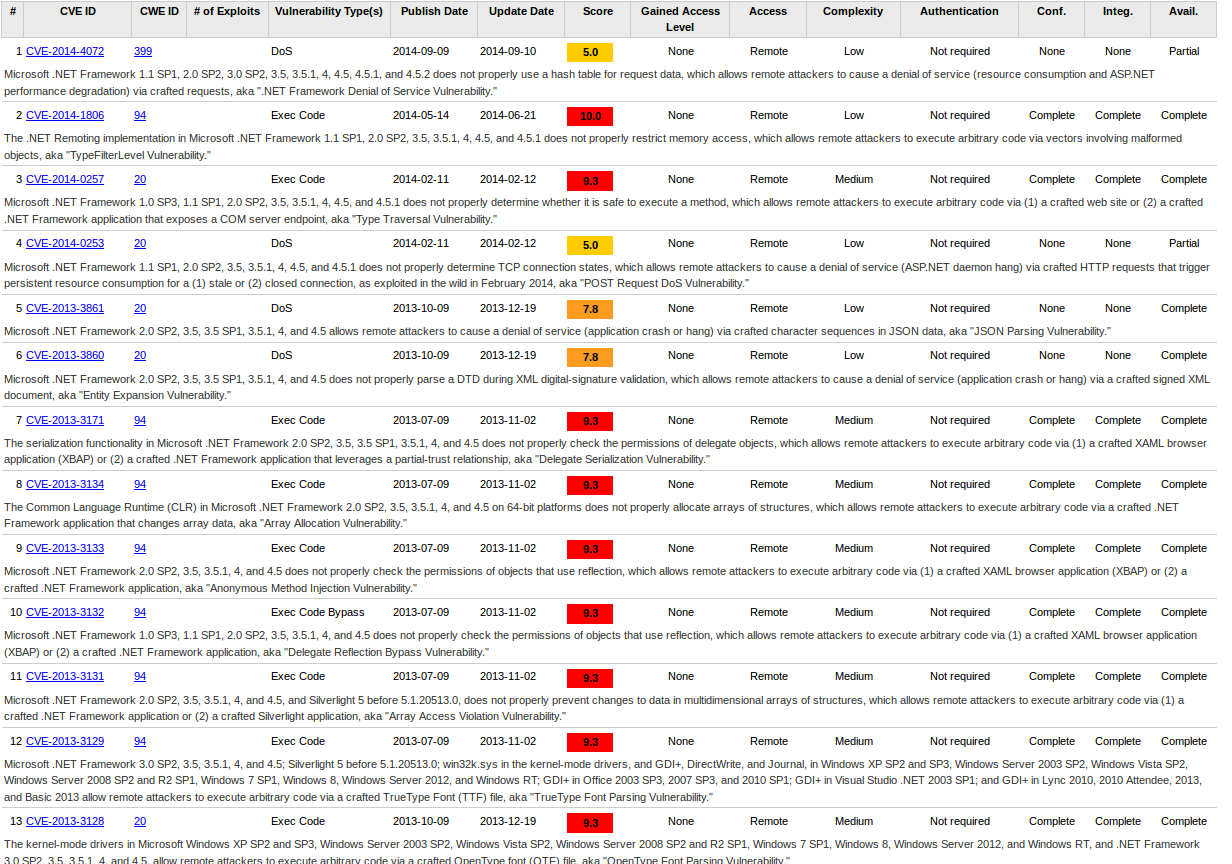
\includegraphics[height=200px]{dotnet_cve.png}

\end{frame}

\begin{frame}
\frametitle{Mono}

Mono provides largely better security guarantees\\
However it pose compatibilities issues since it does support all .NET features\\

    \vfill
    Note: at least mscorelib.dll is needed to run mi.TLS so one shall be carefull with .NET micro frameworks.\\
In particular, mscorelib.dll could introduces security issues

\end{frame}


\section{Possible strategies}

\begin{frame}
\frametitle{Kernel}
Two main candidates :
\begin{itemize}
\item \textbf{Linux} : easier, but not certified.
\item \textbf{Certified micro-kernel} : certified, but may pose compatibilities issues.
\end{itemize}

A first approach could be to develop a prototype on a linux kernel, then try to make it run on a certified kernel, most likely Sel4.

\end{frame}



\begin{frame}
\frametitle{Reusing mi.TLS}
mi.TLS may be used as is for managing TLS protocol\\

However, it does not support SSH, which will likely be used to encapsulate SFTP
Reusing mi.TLS would then mean to adapt implementation and proof for SSH protocol

Still remains the .NET issue :
\begin{itemize}
\item may introduce additional flaws
\item may be hard to port on a micro-kernel
\item we may lose interest of micro-kernel during process
\end{itemize}

\end{frame}


\begin{frame}
\frametitle{Another approach}

D. Cad\'e and B Blanchet have done a similar work on SSH\\

Protocol is specified using CryptoVerif, then automatically translated in OCaml\\

Contrary to mi.TLS, SSH proof is not complete due to CBC-mode\\
However, disabling CBC in our implementation should not cause compatibilities issues

\end{frame}


\begin{frame}
  \frametitle{Advantages}
  This approach has the major advantage that it does not require additional libraries or framework.\\
  This has two main advantages :
  \begin{itemize}
  \item Portage on a micro-kernel should be easier
  \item Less security issues introduced by third-party programs
  \end{itemize}

  this approach can also be applied to TLS, using specifications of mi.TLS

\end{frame}



\begin{frame}
\frametitle{Required Features}
in order to manage protocol rupture, we need various softwares able to interoperate :
\begin{itemize}
  \item SSH server and client
  \item likely TLS server and client
  \item protocol stacks for SFTP, Modbus, OPC-UA
\end{itemize}

We may also need need some \emph{virtualization} tweaks, in order to simulate protocol commands execution

\end{frame}



\begin{frame}
\frametitle{Potential solutions}

Several question need to be discussed :

\begin{itemize}
\item do we separate SSH and TLS (and any other handshake) part from protocol command analysis : we could thus provide a strenghtened external interface, while protocols requests could be analyzed on on a less secured system
\item do we tweak an existing implementation of protocols, or do we develop our own programs tailored to our needs : first option would be quickier and simplier to deploy, while second would lead to better execution time, and we may provide additional security guarantees

\end{itemize}

Concerning the second question, same strategy as for kernel could be adopted : we first develop a working prototype, then try to gradually replace parts with our own implementations

\end{frame}



\end{document}
